\documentclass{ximera}
%% handout
%% nohints
%% space
%% newpage
%% numbers

%% You can put user macros here
%% However, you cannot make new environments

\graphicspath{{./}{firstExample/}{secondExample/}}

\usepackage{url}
\usepackage{tikz}
\usepackage{tkz-euclide}
\usetkzobj{all}


\tikzstyle geometryDiagrams=[ultra thick,color=blue!50!black]
\pgfplotsset{compat=1.8}
  \usepackage[T1]{fontenc}
  \usepackage[utf8x]{inputenc} %% we can turn off input when making a master document

\prerequisites{none}
\outcomes{ximeraLatex}

\title{Wave Functions}

\begin{document}
\begin{abstract}
We meet the sine and cosine functions.
\end{abstract}
\maketitle


We start off by learning about two wave functions called the \emph{sine} and \emph{cosine} functions. In a trigonometry class you would learn a great deal about these functions. In this class we will just learn some of their important characteristics, and we will use them for some limited applications.

Open up the link \link{https://www.desmos.com/calculator/ubhracbupf} in a separate window. Watch the video at  -------------------- Answer each question below.

\begin{exercise}
Compute $\sin\left(\frac{\pi}{6}\right)$.
\begin{solution} 
\begin{hint}
Plug it into desmos or another calculator. 
\end{hint}
\begin{hint}
Be careful, because some calculators are in degree mode. You may need to find a mode setting to change the calculator to be in radian mode.
\end{hint}
$\sin\left(\frac{\pi}{6}\right)=$ \answer{.5}.
\end{solution}
\end{exercise}

\begin{question}
The graph below shows a function of the form $f(x)=a\sin(bx)$, where $b\ge0$. Find the value of $a$ and $b$ to match the graph below.
\begin{image}
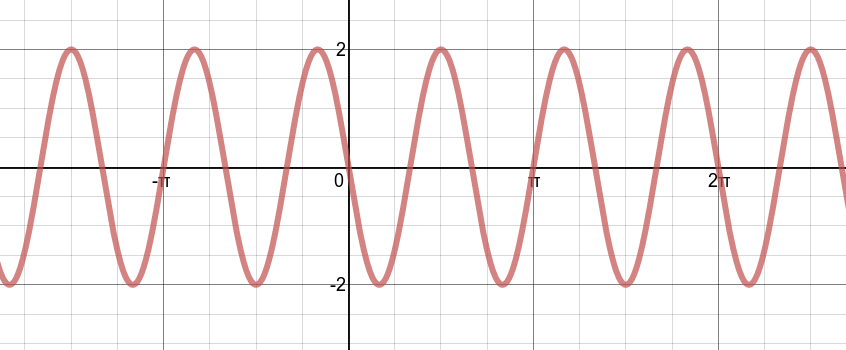
\includegraphics{ParentFunctions2/MoreParentFunctions/mysterysine.png}
\end{image}
\begin{solution}
\begin{hint}
Use Desmos to create the function $f(x)$ with sliders for $a$ and $b$. 
\end{hint}
\begin{hint}
Remember that you can reach the menu to change the $x$-axis labels in desmos by clicking on the wrench.
\end{hint}
In the picture $a=$ \answer{-2} and $b=4$ \answer{3}.
\end{solution}
\end{question}

\begin{question}
In a function of the form $f(x)=a\sin(bx)$ the constant $a$ does what to the graph of $y=\sin(x)$?
  \begin{solution}
    \begin{multiple-choice}
      \choice{---shifts the graph to the right by $a$ units}
      \choice{---shifts the graph upward by $a$ units}
      \choice{---scales the graph horizontally by a factor of $a$}
      \choice[correct]{---scales the graph vertically by a factor of $a$}
    \end{multiple-choice}
    \begin{hint}
    Use Desmos to create the function $f(x)=a\sin(bx)$ with sliders for $a$ and $b$. As you change the value of $a$, what happens to the graph?
    \end{hint}
  \end{solution}
\end{question}

\begin{question}
In a function of the form $f(x)=a\sin(bx)$ the constant $b$ does what to the graph of $y=\sin(x)$?
  \begin{solution}
    \begin{multiple-choice}
      \choice{---shifts the graph to the right by $b$ units}
      \choice{---shifts the graph upward by $b$ units}
      \choice[correct]{---scales the graph horizontally by a factor of $\frac{1}{b}$}
      \choice{---scales the graph vertically by a factor of $\frac{1}{b}$}
    \end{multiple-choice}
    \begin{hint}
    Use Desmos to create the function $f(x)=a\sin(bx)$ with sliders for $a$ and $b$. As you change the value of $b$, what happens to the graph?
    \end{hint}
  \end{solution}
\end{question}

\end{document}